\documentclass[border=3pt]{standalone}
% Shared preamble for every generated figure.
% Matches the report: newtx (Times), greyscale, square boxes.
\usepackage{newtxtext,newtxmath}
% newtx's typewriter (txtt) draws a slashed zero; use Latin Modern instead.
\renewcommand{\ttdefault}{lmtt}
\usepackage{tikz}
\usetikzlibrary{positioning,arrows.meta,calc,fit,backgrounds,shapes.geometric,
                decorations.pathreplacing,decorations.pathmorphing,matrix,patterns}

\definecolor{figgrey}{gray}{0.88}
\definecolor{figmid}{gray}{0.60}
\definecolor{figdark}{gray}{0.35}

\tikzset{
  fig/.style={font=\small},
  box/.style={draw,thick,minimum height=8mm,minimum width=22mm,align=center,
              inner sep=2pt,font=\small},
  greybox/.style={box,fill=figgrey},
  smallbox/.style={draw,minimum height=6mm,minimum width=16mm,align=center,
                   inner sep=2pt,font=\scriptsize},
  ln/.style={-{Stealth[length=2.2mm,width=1.8mm]},thick},
  lnb/.style={{Stealth[length=2.2mm,width=1.8mm]}-{Stealth[length=2.2mm,width=1.8mm]},thick},
  lbl/.style={font=\scriptsize,inner sep=1.5pt},
  note/.style={font=\scriptsize\itshape,inner sep=1.5pt},
}

\begin{document}
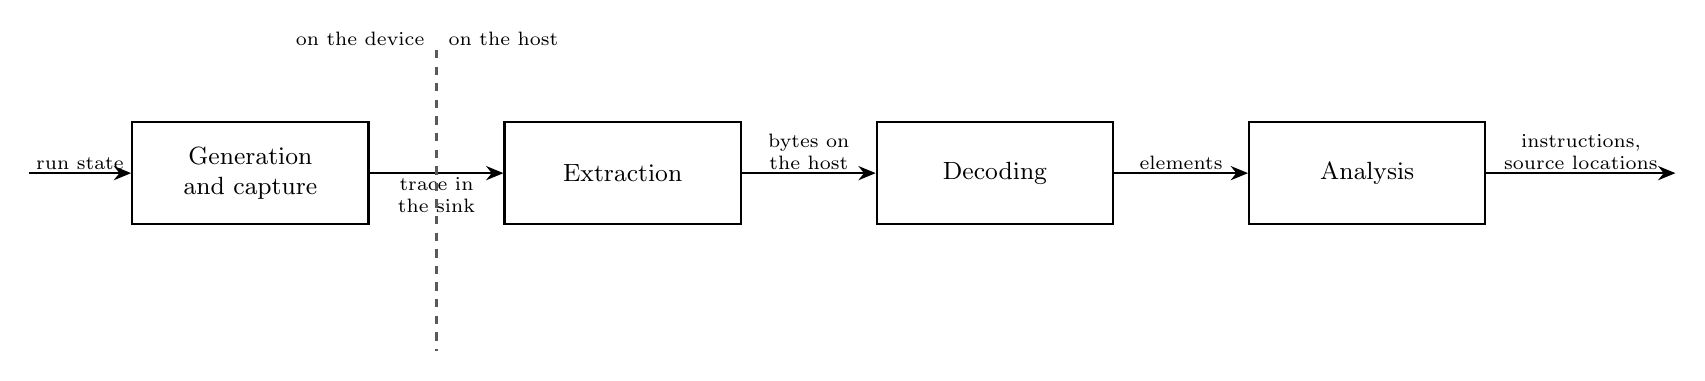
\begin{tikzpicture}[fig,
  st/.style={draw,thick,minimum height=13mm,minimum width=30mm,align=center,font=\small},
  io/.style={font=\scriptsize,align=center,inner sep=1pt},
  dep/.style={font=\scriptsize\itshape,align=center,inner sep=1pt}]

\node[st] (s1) {Generation\\and capture};
\node[st,right=17mm of s1] (s2) {Extraction};
\node[st,right=17mm of s2] (s3) {Decoding};
\node[st,right=17mm of s3] (s4) {Analysis};

\draw[ln] (s1) -- node[io,below]{trace in\\the sink} (s2);
\draw[ln] (s2) -- node[io,above]{bytes on\\the host} (s3);
\draw[ln] (s3) -- node[io,above]{elements} (s4);
\draw[ln] ($(s1.west)-(13mm,0)$) -- node[io,above]{run state} (s1.west);
\draw[ln] (s4.east) -- node[io,above,align=center]{instructions,\\source locations} ++(24mm,0);


\coordinate (bt) at ($(s1.north east)!0.5!(s2.north west)+(0,9mm)$);
\coordinate (bb) at ($(s1.south east)!0.5!(s2.south west)+(0,-16mm)$);
\draw[dashed,figdark,thick] (bt) -- (bb);
\node[lbl,anchor=south east,align=right] at (bt) {on the device\ };
\node[lbl,anchor=south west,align=left]  at (bt) {\ on the host};

\end{tikzpicture}
\end{document}
